\section{Summary}\frame{\sectionpage}

\subsection{Principles}
\begin{frame}{The Four Freedoms of Free Software}
  \begin{itemize}
    \item Freedom 0 is the freedom to run the program as you wish
    \item Freedom 1 is the freedom to study the source code and change it,
      so the program does your computing the way you wish
    \item Freedom 2 is the freedom to help others. That's the freedom to
      make exact copies and redistribute them when you wish
    \item Freedom 3 is the freedom to contribute to your community. That's
      the freedom to make copies of your modified versions, if you have made any,
      and then distribute them to others when you wish
  \end{itemize}
\end{frame}


\begin{frame}{The GNU Project and the Free Software Movement}
  \begin{column}{.45\textwidth}
    \begin{itemize}
      \item Stallman launched the Free Software movement in 1983
      \item He developed GNU - GNU's Not Unix
      \item Hacker spirt to joke around about serious issues
      \item Developed for freedom of users
      \item GNU+Linux or GNU/Linux
    \end{itemize}
  \end{column}
  \begin{column}{0.5\textwidth}\raggedleft{}
    \begin{figure}
      
\includegraphics[width=\textwidth]{images/gnu-linux.jpg}
    \end{figure}
  \end{column}
\end{frame}


\begin{frame}{Free Software and Education}
  \begin{itemize}
    \item Schools must teach exclusively free software
    \item Teaching windows teaches dependence
    \item To become a good programmer, one must read lots of code
    \item Free software fosters sharing and helping
  \end{itemize}
\end{frame}


\subsection{Threats to Freedom}
\begin{frame}{Surveillance}
  \begin{column}{0.45\textwidth}
    \begin{itemize}
      \item Can record anything on a computer
      \item Amazon users identify selves when buying books
      \item Mobile phones transmit location
      \item Need control over software
      \item Computer surveillance centralizes information
    \end{itemize}
  \end{column}
  \begin{column}{0.5\textwidth}\raggedleft{}
    \begin{figure}
      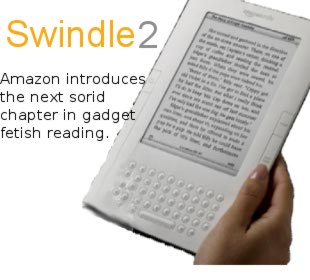
\includegraphics[width=\textwidth]{images/swindle.jpg}
    \end{figure}
  \end{column}
\end{frame}

\begin{frame}{Censorship}
  \begin{column}{0.45\textwidth}
    \begin{itemize}
      \item Arbitray shutdown of sites in Spain
      \item Denmark secretly blocked sites
      \item A country that imposes censorship is not
        \begin{itemize}
          \item free
          \item legitamte
        \end{itemize}
    \end{itemize}
  \end{column}
  \begin{column}{0.5\textwidth}\raggedleft{}
    \begin{figure}
      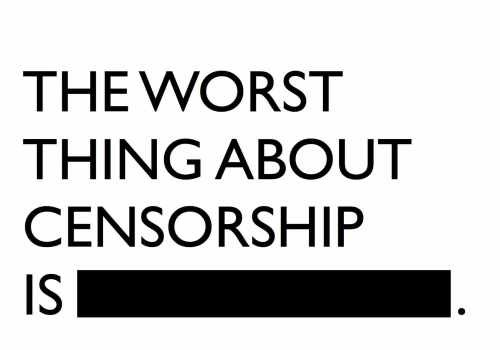
\includegraphics[width=\textwidth]{images/censorship.jpg}
    \end{figure}
  \end{column}
\end{frame}

\begin{frame}{Restricted Data Formats}
  \begin{itemize}
    \item Prevents interoperability
    \item DRM is digital handcuffs
    \item Only happens in non-free software
    \item VC1, Flash, MP3
  \end{itemize}
\end{frame}

\begin{frame}{Software That Isn't Free}
  \begin{itemize}
    \item Free as in {\it libre\/}
    \item Free software respects a user's freedom
    \item The user controls free software
    \item Backdoor
  \end{itemize}
\end{frame}

\begin{frame}{Internet Services}
  \begin{itemize}
    \item Server could abuse data or take control
    \item Never trust data to a US company - Patriot Act
    \item Do things remotely with your own server
    \item Doing things digitally should not require loss of rights
  \end{itemize}
\end{frame}

\begin{frame}{Computers for Voting}
  \begin{itemize}
    \item Can't trust computers for voting
    \item Neither free or non-free software can be used
    \item If non-free software is used, company controls voting
    \item If free software is used, whoever runs the machine is in control
    \item Ballots can't be recounted with digital voting
  \end{itemize}
\end{frame}

\begin{frame}{The War on Sharing}
  \begin{itemize}
    \item Technology makes it easy to copy published works
    \item Those who have power over distribution do not want sharing
    \item Suing teenages for hundreds of thousands of dollars for sharing
    \item DMCA makes free software that circumvents DRM illegal
    \item Streaming media requires proprietary software
    \item Users should have their own copy of media
  \end{itemize}
\end{frame}

\begin{frame}{Rights in Cyberspace}
  \begin{itemize}
    \item No firm right to do things in cyberspace
    \item Need support of ISP to have website
    \item Need support of payment company to get paid
    \item US government had Amazon cut off service to WikiLeaks
    \item Also had PayPal cut service from WikiLeaks
    \item Need to have same rights in physical and virtual worlds
  \end{itemize}
\end{frame}
